\documentclass[10pt]{article}
\usepackage[margin=0.72in]{geometry}
\usepackage[T1]{fontenc}
\usepackage{lmodern}
\usepackage{microtype}
\usepackage{graphicx}
\usepackage{booktabs}
\usepackage{tabularx}
\usepackage{array}
\usepackage[table]{xcolor}
\usepackage{enumitem}
\usepackage[hidelinks]{hyperref}
\usepackage{fancyhdr}
\usepackage{amsmath}
\usepackage{amssymb}

\definecolor{navy}{HTML}{183153}
\definecolor{teal}{HTML}{0F6B78}
\definecolor{pale}{HTML}{EEF5F6}
\definecolor{warn}{HTML}{FFF2CC}
\definecolor{bad}{HTML}{FCE8E6}
\definecolor{good}{HTML}{E6F4EA}
\newcommand{\code}[1]{\texttt{\detokenize{#1}}}
\newcommand{\status}[1]{\textbf{\color{teal}#1}}
\newcolumntype{Y}{>{\raggedright\arraybackslash}X}
\setlist[itemize]{leftmargin=1.25em,itemsep=2pt,topsep=3pt}
\setlength{\parindent}{0pt}
\setlength{\parskip}{5pt}
\pagestyle{fancy}
\fancyhf{}
\lhead{Luo--Maunsell environment audit}
\rhead{18 July 2026}
\cfoot{\thepage}

\begin{document}

\begin{center}
{\LARGE\bfseries\color{navy} Luo \& Maunsell reward-dissociation experiment}\\[4pt]
{\large Primary-paper verification, repository audit, and corrected environment report}\\[7pt]
{\small 18 July 2026 \quad $\cdot$ \quad AttentionManuscript / RViT+ battery}
\end{center}

\vspace{4pt}
\colorbox{pale}{\parbox{0.96\linewidth}{
\textbf{Determination.} The cited first author is \textbf{Tianming Z. Luo}; this report did not independently verify a preferred personal form beyond the publication metadata. The task is the one the question anticipated: location-specific \textbf{hit} and \textbf{correct-rejection} rewards were manipulated to separate changes in signal-detection sensitivity ($d'$) from shifts in decision criterion ($c$). The direct protocol for \code{envs/luo2015.py} is Luo \& Maunsell (2015), recorded in visual area V4. Luo \& Maunsell (2018) is a related lateral-prefrontal-cortex extension, not a replacement protocol.
}}

\section{Bottom line}

\begin{itemize}
\item The repository previously contained four completed 20,000-iteration \code{luo_maunsell_*} final checkpoints (sensitivity/criterion $\times$ affine/cross-attention) and four rolling \code{latest} checkpoint files. All eight obsolete weight files were deleted on 18 July 2026. Their \code{metrics.csv} logs remain only as historical records of the preliminary, cued task; they are not corrected Luo--Maunsell evidence.
\item A newer cue-free \code{luo2015_*} environment existed, but before this audit it still omitted the active second test, randomized the orientation pair between trials, used incomplete reward schedules, treated premature declarations as false alarms, and rewarded passive waiting as a correct rejection.
\item The environment and analysis have now been corrected to implement a close, scaled analogue of the published trial and reward mechanics. Focused verification passes (41 tests plus live outcome exercise); the complete repository suite reached 312 passes and three unrelated Python-3.9 compatibility failures.
\item \textbf{No production corrected \code{luo2015_*} matrix has yet been trained.} One equal-reward-parent cell and four one-iteration child cells were exercised on MPS; rolling and final saves produced ten physical checkpoint files. They verify plumbing only. The transition system is ready for a production-scale computational analogue after the analysis safeguards below are fixed, but no local behavioral replication or dissociation has been demonstrated.
\end{itemize}

\section{What the papers actually did}

\subsection{Primary 2015 V4 study}
Two full-contrast Gabor samples were shown simultaneously at opposite locations. In a session, each location used only two possible orientations, randomized independently across trials. For the neuronal experiment, the receptive-field stimulus orientation was set $90^\circ$ from the opposite-hemifield stimulus to reduce feature-attention effects. After a delay, one location was tested. The monkey reported an orientation change by making a saccade to the test. If the first test was unchanged, a subsequent guaranteed changed test required a response; trials without that response were excluded. This made a correct rejection an \emph{verified withholding} at the first test rather than passive non-response.

The experiment counterphased reward contingencies across locations and across task conditions. A location carrying one contingency in condition A carried the opposite contingency in condition B. No visual value cue identified the condition; the animal learned it from reward history. Sessions began with a small number of priming trials, and behavioral SDT measures were computed by test location.

\begin{table}[ht]
\centering
\small
\caption{Fixed local reward parameters reconstructed from the published session-average ratios. ``Mean'' is the arithmetic mean of the hit and correct-rejection magnitudes. The paper used dynamically titrated liquid rewards averaging about 150~$\mu$L; the code uses dimensionless, fixed values and is not a literal reward-volume reproduction.}
\begin{tabularx}{\linewidth}{@{}l l c c c c@{}}
\toprule
Session & Location role & Mean & H:CR & Hit reward & CR reward \\
\midrule
Sensitivity & high-value / high-$d'$ & 5.00 & 0.7 & 4.12 & 5.88 \\
Sensitivity & low-value / low-$d'$ & 1.00 & 1.1 & 1.05 & 0.95 \\
Criterion & low-$c$ (liberal) & 0.90 & 1.5 & 1.08 & 0.72 \\
Criterion & high-$c$ (conservative) & 1.00 & 0.5 & 0.67 & 1.33 \\
\bottomrule
\end{tabularx}
\end{table}

The signal-detection quantities are
\[
 d' = z(\mathrm{HR}) - z(\mathrm{FAR}), \qquad
 c = -\tfrac{1}{2}\left[z(\mathrm{HR})+z(\mathrm{FAR})\right].
\]
Increasing both hit and false-alarm rates shifts $c$ in the liberal direction; increasing hit rate while lowering false-alarm rate increases $d'$. The local hypothesis is that the H:CR ratio changes response bias and that a between-location difference in average correct-outcome reward changes learned spatial sensitivity. The latter is a finite-policy optimization hypothesis, not a direct implementation of a formal resource-allocation mechanism.

\subsection{Related 2018 LPFC study}
The 2018 experiment applied the same conceptual dissociation in lateral prefrontal cortex. Its abstract reports robust LPFC response modulations in both the criterion and sensitivity conditions, with task-related activity tracking the specific behavioral component manipulated. It is relevant context for neural interpretation, but \code{luo2015.py} remains keyed to the 2015 V4 protocol; no stronger neural claim is inferred here.

\section{Repository state before correction}

\begin{tabularx}{\linewidth}{@{}p{0.25\linewidth}Y Y@{}}
\toprule
Artifact & What existed & Scientific status \\
\midrule
\code{envs/tasks.py} / \code{luo_maunsell_*} & Generic battery task: a visible per-trial cue selected the high-value location; criterion H:CR rewards were global rather than spatially counterphased. & Preliminary analogue; not the cue-free published method. \\
\code{battery_sweep_results} & Historical \code{metrics.csv} logs remain; all four final and four rolling \code{luo_maunsell_*} weight files were deleted. & Trained on the preliminary task. The retained scalar logs have no corrected task lineage or trial-level SDT outcomes and are non-evidential. \\
\code{envs/luo2015.py} & Cue-free two-location sample/test task, registered as \code{luo2015_sensitivity} and \code{luo2015_criterion}. & Better identity, but protocol gaps made its CR and reward logic scientifically incorrect. \\
\code{luo2015_analysis} & Offline hit/FA and $d'/c$ readout. & Counted any no-change declaration as an FA and did not enforce second-test engagement exclusions. \\
Corrected checkpoints & Five logical one-iteration canary cells (one parent, four children), each with rolling and final saves; no production matrix. & Ten physical checkpoint files, all plumbing-only; the corrected experiment has not produced behavioral evidence. \\
\bottomrule
\end{tabularx}

\subsection{Why the deleted checkpoints could not answer the scientific question}
Before deletion, inspection showed that each final checkpoint contained an iteration value of 20,000, the preliminary task name, model constructor arguments, and the learned state dictionary. It did not contain the environment configuration, the spatial reward table, condition-switch history, trial-level outcomes, an SDT summary, or producer-source hashes. A weight file by itself therefore could not establish whether sensitivity or criterion moved in the intended direction.

More importantly, the embedded task identity was {\small\code{luo_maunsell_sensitivity}} or {\small\code{luo_maunsell_criterion}}, not the corrected \code{luo2015_*} identity. In the old sensitivity environment, the high-value location was set to the visible cue location on each trial. In the old criterion environment, the H:CR ratio was global rather than assigned oppositely across the two locations. Those are substantive experimental differences, not naming differences. Any plots or aggregate logs derived from those deleted checkpoints remain preliminary historical artifacts and must not be relabeled as corrected Luo--Maunsell results.

Deletion was restricted to the two \code{.pt} files in each of four preliminary directories: \path{luo_maunsell_sensitivity_affine_ew}, \path{luo_maunsell_sensitivity_crossattn1}, \path{luo_maunsell_criterion_affine_ew}, and \path{luo_maunsell_criterion_crossattn1}. In each directory, both its named \path{*_final.pt} file and \path{rvit_plus_rl_latest.pt} were removed. The four \code{metrics.csv} files and the derived aggregate-metrics inventories that reference them were retained for audit history. Twelve unrelated checkpoint files in the same pod were left untouched, and a post-deletion search found no remaining \path{luo_maunsell*.pt} file there.

\section{Paper-to-code correction map}

\small
\begin{tabularx}{\linewidth}{@{}p{0.18\linewidth}p{0.24\linewidth}Y p{0.14\linewidth}@{}}
\toprule
Protocol element & Before audit & Corrected implementation & Fidelity \\
\midrule
Value information & New environment had no cue, but reward schedules were incomplete. & No cue; \code{condition_loc} / \code{set_condition()} swaps a hidden reward table across locations. & Close \\
Two orientations & Base angle re-randomized each trial. & Two fixed orientation values per location within a session; sampled member randomized per trial. The two location bases are independent and do not enforce the paper's $90^\circ$ cross-hemifield control. & Partial \\
First test & One test persisted from frame 3 onward. & First-test response window is frames 3--4. & Scaled \\
Correct rejection & Passive waiting until trial end earned CR reward. & Withhold to an unchanged first test, then declare to a changed second test at frame 6. & Method-matched \\
Exclusions & Premature no-change declarations became FAs; no second-test failure class. & Fixation breaks and second-test misses are separately labeled and excluded from SDT; the analyzer now preserves both counts by location/status. & Close \\
Sensitivity rewards & Same H/CR reward at each location. & Fixed, normalized 5:1 mean-reward contrast with published average 0.7 and 1.1 H:CR ratios; counterphased, without online titration. & Fixed-ratio analogue \\
Criterion rewards & One global H:CR pair. & Fixed spatial 1.5 versus 0.5 H:CR ratios; low-$c$ mean is 90\% of high-$c$ mean; counterphased, without online titration. & Fixed-ratio analogue \\
Fixation & No explicit central fixation. & Central white fixation is present throughout the rendered trial. & Close \\
Difficulty & Curriculum default could change the orientation pair. & Protocol defaults to fixed $\theta$; curriculum remains optional only when explicitly requested. & Method-matched \\
Checkpoint safety & Subclass reward/condition state absent; source hash omitted Luo file. & Environment state binds session, condition, reward table, and orientation bases; trainer hashes \code{envs/luo2015.py}. & Stronger \\
Timing/apparatus & Seven abstract frames, 50-pixel image, binary action. & Explicit scaled timeline retained; action 1 stands in for a test-directed saccade. & Analogue \\
\bottomrule
\end{tabularx}
\normalsize

\clearpage
\section{Current local task: exact interaction contract}

\subsection{Biological anchor and scope of the local analogue}

The governing experiment is Luo and Maunsell's 2015 V4 dissociation task, not the earlier generic battery task and not the 2018 LPFC extension. In the biological experiment, the monkey first fixated for 400--600~ms. Two full-contrast sample Gabors then appeared on opposite sides of fixation for 200~ms, followed by a 200--300~ms delay. A single first test appeared for 200~ms at a randomly selected sample location. Its probability of differing from the sample at that location was 0.5. A changed first test required a saccade within 100--500~ms. An unchanged first test required withholding that saccade and then responding to a guaranteed changed second test at the same location. Failure to answer the second test was rare in the paper and excluded from analysis.

The local environment preserves that decision structure while compressing physical time into seven logical frames. It is therefore a \emph{scaled computational analogue}, not a millisecond-exact reproduction of the monkey apparatus. The local agent has recurrent state within one trial, but that state is reinitialized at every environment reset. Consequently, the planned paired optimization experiment compares finite-budget policies trained under fixed reward schedules. It does not establish global policy optima and does not model the monkey's adaptation across the paper's alternating 240--360-trial blocks, online reward titration, or priming trials.

\subsection{Registration, geometry, and trial randomization}

The task registry exposes two names, \code{luo2015_sensitivity} and \code{luo2015_criterion}. Both instantiate the same \code{LuoMaunsell2015Env} transition system. The names select different reward tables; they do not change the images, action space, trial probabilities, or outcome definitions.

At every reset, the environment constructs one trial as follows.
\begin{enumerate}[leftmargin=1.5em,itemsep=3pt]
\item The observation is a 50$\times$50 RGB array on a $2\times2$ spatial grid. Only grid locations 0 (top-left) and 3 (bottom-right) contain Gabors. Locations 1 and 2 remain black except for any central fixation pixels at the shared grid boundary. A white $2\times2$ central fixation point is drawn on every logical frame.
\item Each active location $i\in\{0,3\}$ has a session-fixed base $b_i$ and current pair $\{b_i,b_i+\theta\}$. At environment construction, $b_0$ and $b_3$ are drawn independently from $\operatorname{Uniform}[0^\circ,180^\circ)$; there is no constraint on their separation and therefore no implementation of the paper's $90^\circ$ control. On each trial, the sample orientation at each location is chosen independently and uniformly from its current pair. The base orientations remain fixed; only the parent curriculum can reduce $\theta$ between trial windows.
\item The tested location is sampled uniformly from locations 0 and 3. Independently, the trial is sampled as changed or unchanged with probability 0.5.
\item On a changed trial, the first test uses the \emph{other} member of the tested location's orientation pair. On an unchanged trial, it repeats the sampled member. The second test on an unchanged trial always uses the other member and is therefore guaranteed to differ by exactly $\theta$ in nominal orientation.
\item Stimulus position identifies which location is being tested, but there is no separate cue identifying the high-value location, reward condition, or child identity. The reward condition is hidden from the pixels and fixed for the lifetime of one trained child agent.
\end{enumerate}

The image geometry is not apparatus-matched. The paper placed stimuli on opposite sides of fixation at calibrated visual eccentricities, whereas the local renderer places them diagonally in the top-left and bottom-right cells of a 50-pixel image. The local claim therefore concerns the sample/test decision and reward contingencies, not retinotopic equivalence to the monkey display.

The default renderer adds two forms of sensory variability. Before drawing a Gabor, it adds zero-mean Gaussian orientation noise with standard deviation $5^\circ$. It also adds independent uniform pixel noise from $-0.11$ to $0.11$ inside the Gabor aperture. These two noise choices are local model-side approximations; their distributions and magnitudes were not taken from Luo and Maunsell's apparatus specification. Frames 0 and 1 therefore show the same nominal sample orientations with newly rendered noise, and frames 3 and 4 likewise show the same nominal first test with newly rendered noise. The declared Gym observation box is $[-1,1]$, although the post-noise Gabor array is not clipped after adding pixel noise; the executable renderer, rather than the nominal box bound, is the exact source of the values consumed by the model.

\subsection{What is shown at every timestep}

The planned full matrix uses \code{T=7} and \code{frame_repeat=1}, so one logical frame equals one policy decision. The observation in the table is the frame visible \emph{before} the action is selected. Internally, \code{step(action)} classifies the action against that current frame, increments the timestep, and returns the next observation. A terminal outcome stops the episode immediately.

\small
\renewcommand{\arraystretch}{1.12}
\begin{tabularx}{\linewidth}{@{}p{0.07\linewidth}p{0.25\linewidth}Y Y@{}}
\toprule
Frame & Pixels shown before action & Action 0: wait/withhold & Action 1: declare/respond \\
\midrule
0 & Both sample Gabors at locations 0 and 3; central fixation; no cue. & Continue to frame 1 with zero reward on either trial type. & Terminal \emph{fixation break}, zero reward, invalid for SDT. \\
1 & Both samples again at the same nominal orientations, with fresh renderer noise; fixation. & Continue to blank delay frame 2 with zero reward. & Terminal \emph{fixation break}, zero reward, invalid for SDT. \\
2 & Black field plus central fixation only; this is the scaled delay. & Continue to first-test frame 3 with zero reward. & Terminal \emph{fixation break}, zero reward, invalid for SDT. \\
3 & First test at the randomly selected location; the other three cells are black; fixation remains. & Continue to frame 4 with zero reward on both changed and unchanged trials. & Changed trial: terminal \emph{hit}, valid for SDT, location-specific hit reward. Unchanged trial: terminal \emph{false alarm}, valid for SDT, zero reward. \\
4 & The same nominal first test appears again with fresh renderer noise; fixation remains. & Changed trial: terminal \emph{miss}, valid for SDT, zero reward. Unchanged trial: continue to gap frame 5 with zero reward. & Changed trial: terminal \emph{hit} with hit reward. Unchanged trial: terminal \emph{false alarm} with zero reward. Both are valid for SDT. \\
5 & Black inter-test gap plus fixation. This frame is reachable only after withholding on an unchanged first test. & Continue to second-test frame 6 with zero reward. & Terminal \emph{fixation break}, zero reward, invalid for SDT. A changed trial cannot reach this frame in live execution because it ended as a hit or miss by frame 4. \\
6 & On an unchanged trial, a guaranteed changed second test at the same tested location; fixation remains. & Terminal \emph{second-test miss}, zero reward, invalid for SDT and excluded. & Terminal \emph{correct rejection}, valid for SDT, location-specific correct-rejection reward. A changed trial cannot normally reach this frame. \\
\bottomrule
\end{tabularx}
\normalsize

The binary action does not encode a spatial choice. Action 1 means ``respond to the currently presented test,'' analogous to a test-directed saccade; the test's location is supplied by the image. Before the first test and during the inter-test gap, the same action is treated as a fixation break. There is no negative punishment: misses, false alarms, fixation breaks, and second-test misses all receive zero. Only hits and verified correct rejections receive positive reward.

\subsection{Complete outcome partition and SDT denominators}

\begin{tabularx}{\linewidth}{@{}p{0.18\linewidth}p{0.31\linewidth}p{0.12\linewidth}Y@{}}
\toprule
Outcome & Exact action history at the decisive frame & SDT status & Reward and analysis role \\
\midrule
In progress & Action 0 before a terminal rule is reached. & Not yet classified & Zero reward; the trial continues and recurrent state is carried to the next frame. \\
Hit & Changed first test; action 1 at frame 3 or 4. & Valid & Hit reward for the tested location; contributes to the hit-rate numerator and change-trial denominator. \\
Miss & Changed first test; no action 1 by the end of frame 4. & Valid & Zero reward; contributes only to the change-trial denominator. \\
False alarm & Unchanged first test; action 1 at frame 3 or 4. & Valid & Zero reward; contributes to the false-alarm numerator and no-change denominator. \\
Correct rejection & Unchanged first test; action 0 at frames 3--5, then action 1 to the changed second test at frame 6. & Valid & CR reward for the tested location; contributes to the no-change denominator. This active verification is the local counterpart of the paper's engagement check. \\
Fixation break & Action 1 at frame 0, 1, 2, or reachable frame 5. & Excluded & Zero reward; labeled separately in live and offline output and omitted from ordinary hit/false-alarm denominators. \\
Second-test miss & Unchanged first test; action 0 through frame 6. & Excluded & Zero reward; labeled separately in live and offline output and omitted from ordinary SDT denominators, matching the paper's exclusion of failures to answer the changed second test. \\
\bottomrule
\end{tabularx}

After exclusions, the local analysis computes $\mathrm{HR}=H/N_H$ with $N_H=H+M$ and $\mathrm{FAR}=FA/N_F$ with $N_F=FA+CR$, separately by tested location. Before applying $z$, it clips HR to $[1/(2N_H),1-1/(2N_H)]$ and FAR independently to $[1/(2N_F),1-1/(2N_F)]$. It then computes $d'=z(\mathrm{HR})-z(\mathrm{FAR})$ and $c=-\tfrac12[z(\mathrm{HR})+z(\mathrm{FAR})]$. During deterministic evaluation, the model emits two action logits at every frame; the evaluator takes their argmax, records the first frame assigned action 1, and applies the live-compatible six-outcome partition. For a changed video, a first declaration after frame 4 remains a miss because live execution would already have terminated at frame 4.

The executable step interface returns \code{(next_obs, reward, done, info)}. The \code{info} dictionary exposes the current orientation magnitude \code{theta}, binary \code{correct} flag, tested grid location \code{test_loc}, ground-truth change flag \code{change}, condition location \code{high_value_index}, categorical \code{outcome}, and Boolean \code{valid_sdt}. Thus exclusions do not have to be reconstructed from reward zero. The corrected offline summary now reports fixation-break and second-test-miss counts separately overall and within every tested-location/status cell, together with valid fractions.

\subsection{Environment reward schedules supplied to the trainer}

The raw environment table reconstructs the published average between-location and H:CR ratios as fixed dimensionless values; it does not reproduce liquid volumes or the paper's online titration. The paired matrix then applies one positive session-wide scale that sets the arithmetic mean of the four correct-outcome magnitudes in each session type to one. This is not a behavior-weighted expected-reward normalization. The scale preserves every within-session ratio. Planned runs use $\gamma=1$, so a CR delivered at frame 6 is not discounted relative to a hit delivered at frame 3 or 4.

\small
\begin{tabularx}{\linewidth}{@{}p{0.17\linewidth}p{0.16\linewidth}p{0.16\linewidth}p{0.07\linewidth}p{0.16\linewidth}Y@{}}
\toprule
Local schedule / location & Published average targets & Fixed raw H / CR & Scale & Trainer H / CR & Local hypothesis \\
\midrule
Sensitivity favored & Mean 5.0; H:CR 0.7 & 4.1176 / 5.8824 & $1/3$ & 1.3725 / 1.9608 & Higher learned $d'$ than the paired location. \\
Sensitivity other & Mean 1.0; H:CR 1.1 & 1.0476 / 0.9524 & $1/3$ & 0.3492 / 0.3175 & Lower-value member of the spatial contrast. \\
Criterion low-$c$ & Mean 0.9; H:CR 1.5 & 1.0800 / 0.7200 & $1/0.95$ & 1.1368 / 0.7579 & More liberal learned criterion. \\
Criterion high-$c$ & Mean 1.0; H:CR 0.5 & 0.6667 / 1.3333 & $1/0.95$ & 0.7018 / 1.4035 & More conservative learned criterion. \\
\bottomrule
\end{tabularx}
\normalsize

The condition location is counterphased. In a \code{condition_loc=0} child, location 0 receives the favored sensitivity schedule or the low-$c$ criterion schedule and location 3 receives its counterpart. In a \code{condition_loc=3} child, those assignments swap. The equal-reward parent---called ``neutral'' only in directory and manifest identifiers---uses $H=CR=1$ at both locations; it is an initialization control, not a zero-reward or behaviorally neutral policy.

\subsection{Implemented paired matrix and exact training contract}

The executable launcher is \path{RViT_plus_paper_jepa_grid9/experiments/luo2015_episodic/run_matrix.py}; the independent evidence validator is the neighboring \path{analyze_matrix.py}. They separate biological task mechanics from the local causal optimization comparison. The planned hierarchy is:

\begin{enumerate}[leftmargin=1.5em,itemsep=4pt]
\item \textbf{One equal-reward parent per seed.} The parent starts from a fresh random initialization with $H=CR=1$ at both locations. The planned full budget is 20,000 trainer iterations with eight newly sampled episodes each, or 160,000 episodes. Curriculum starts at $\theta=65^\circ$. After each non-overlapping window of 1,000 valid SDT trials, it computes $(H+CR)/(H+M+FA+CR)$; at 85\% or better, $\theta$ drops by $3^\circ$ to a floor of $18^\circ$. Exclusions do not enter the window. Reaching the floor does not stop the fixed budget early.
\item \textbf{One hard parent gate.} At $18^\circ$, the parent is tested on 100 trials in each of four location-by-change-status cells, for 400 total. Change accuracy is $H/(H+M)$ and engagement is $(H+M)/100$; no-change accuracy is $CR/(FA+CR)$ and engagement is $(FA+CR)/100$. Every cell must reach 75\% accuracy and 90\% engagement. The deterministic bank uses seed $20260717+s$ for parent seed $s$ and draws one fixed orientation base at each location. A failure aborts launch before any child for that seed; the present contract has no declared replacement-seed rule.
\item \textbf{Four weight-identical children per seed.} Sensitivity-location-0, sensitivity-location-3, criterion-location-0, and criterion-location-3 strictly load the exact parent model state and verify its byte hash. ``Identical'' applies at the fork only: every child then becomes a separate policy. Warm start does \emph{not} transfer optimizer, PAC target-network, JEPA-teacher, replay-buffer, RNG, or environment state; these start fresh, while the parent model weights (including learned heads) transfer. Every child uses the same VDA/RViT \code{affine_ew} architecture, fixed $\theta=18^\circ$, no curriculum, no value cue, one hidden reward table, and 20,000 iterations (160,000 newly sampled episodes).
\item \textbf{Implemented trainer, not reward-only PPO.} The historical API names it PPO, but the update is a PAC-style categorical actor loss: MPO cross-entropy blended with behavior cloning, plus a distributional QR-DQN value loss and entropy regularization. The configured run also uses prioritized episode replay and temporal JEPA/DINO self-distillation with coefficient 0.5. Default material settings are learning rate $3\times10^{-4}$, four update epochs, value coefficient 0.5, entropy coefficient 0.01, MPO temperature 0.1, BC blend 0.1, EMA PAC target decay 0.995, replay capacity 1,000 with four replay episodes, and a 20-iteration forced-wait critic/representation burn-in. The reward table is the between-child intervention, not the trainer's only loss. Recurrent state spans at most the seven frames of one episode and resets before the next.
\item \textbf{Matched deterministic evaluation.}\newline The analyzer verifies and loads each manifest-recorded final child checkpoint---iteration 19,999 under the default budget---after checking file hash, parent lineage, protocol, and producer hashes. At $18^\circ$, the default bank uses seed 20260717 and 200 trials in each location-by-status cell, for 800 total. One environment instance draws one fixed orientation base at each location. The exact tensor bank is reused across every child and seed, with argmax actions. It is generated separately from the parent gate but is not guaranteed stimulus-disjoint: the seed-0 gate and final bank share the default base seed while requesting different sizes. The analyzer now preserves both exclusion categories by location/status and excludes them from ordinary SDT denominators.
\item \textbf{Paired seed-level inference.} Counterphasing removes a fixed location effect only if the equal-reward parent has no material location imbalance, which must be checked empirically. The location-0 minus location-3 contrast under \code{condition_loc=0} is differenced against the same contrast under \code{condition_loc=3}, then halved. The experiment contract prespecifies positive sensitivity-session $\Delta_{\mathrm{DID}}(d')$ and negative criterion-session $\Delta_{\mathrm{DID}}(c)$. The planned seeds are 0--4; these five independent parent lineages, not 800 evaluation trials, are the optimization replicates. With $n=5$, bootstrap intervals are exploratory rather than confirmatory.
\end{enumerate}

This structure asks a narrower question than the monkey block-switching experiment: whether fixed Luo--Maunsell-inspired reward schedules produce directional differences between finite-budget recurrent visual policies. A continuously learning agent would be required for a claim about adaptation speed or inference of an unobserved reward block.

\colorbox{warn}{\parbox{0.96\linewidth}{
\textbf{Analysis safeguards not yet enforced.} Before any production SDT claim, the contract must freeze numerical child-level rules for the minimum $N_H$ and $N_F$, maximum exclusion fraction in each child$\times$location$\times$status cell, and treatment of raw HR or FAR equal to 0 or 1 after finite-rate correction. It must also freeze failed-seed replacement/exclusion rules, the seed count, uncertainty procedure, directional decision threshold, and equivalence bounds for ``no cross-effect.'' The analyzer now emits the necessary separate exclusion counts and valid fractions, but it does not yet block evidence on these numerical rules. Until they are encoded and tested, its $d'$ and $c$ output is descriptive only.
}}

\section{Corrected environment visualization}
Figure~\ref{fig:sample} holds the rendered trial state fixed to show that changing the reward condition does not itself alter the pixels: only the reward table differs. This counterfactual illustration must not be read as a claim that independently trained children consume identical videos in the same order; exact stimulus matching is guaranteed only by the common evaluation bank. Figure~\ref{fig:second} shows the guaranteed changed second test used to validate a correct rejection.

\begin{figure}[ht]
\centering
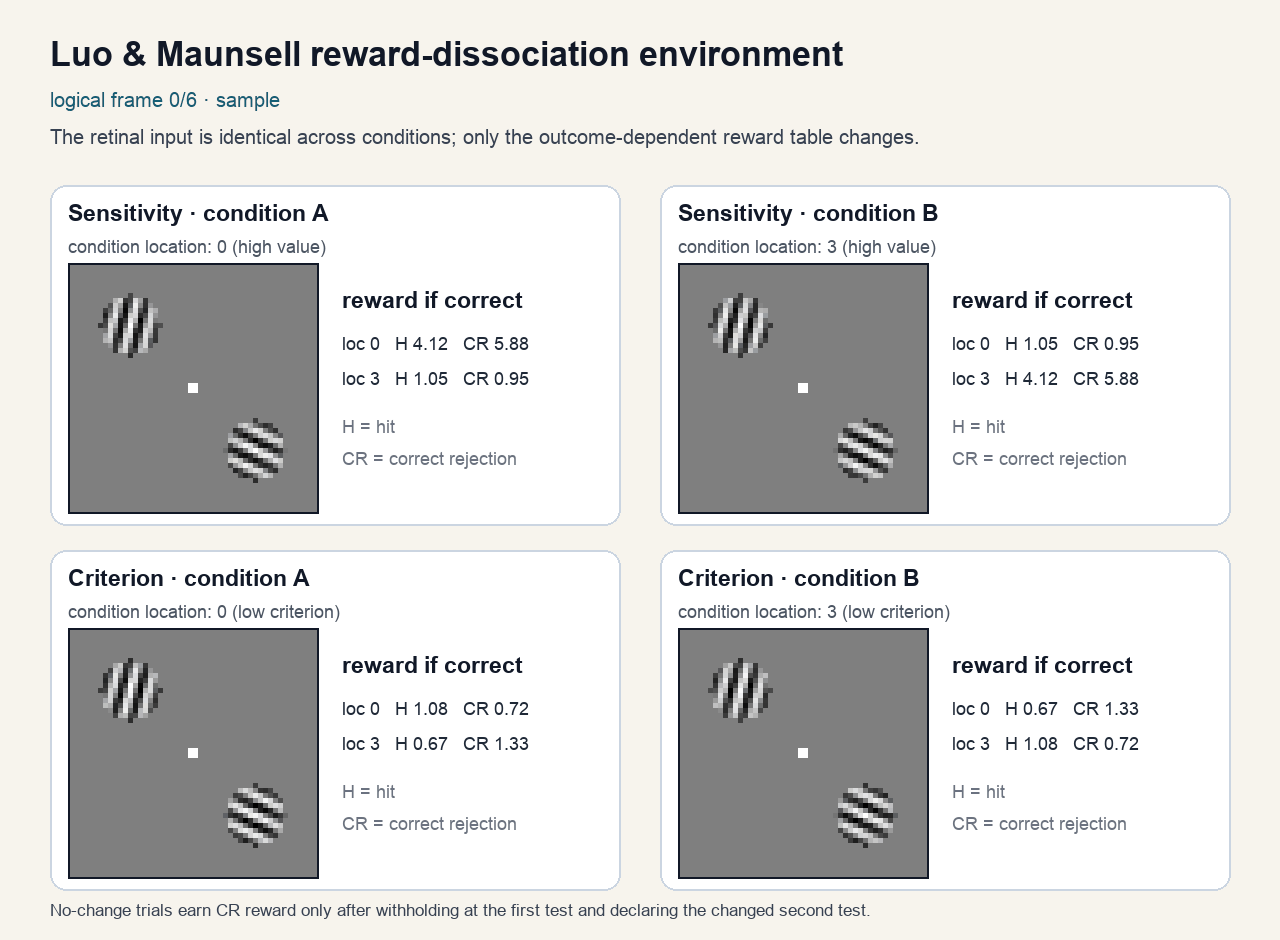
\includegraphics[width=0.91\linewidth]{luo_maunsell_protocol_frame_0.png}
\caption{Sample frame. Reward annotations are outside the agent observation; there is no condition cue in the 50$\times$50 input.}
\label{fig:sample}
\end{figure}

\begin{figure}[ht]
\centering
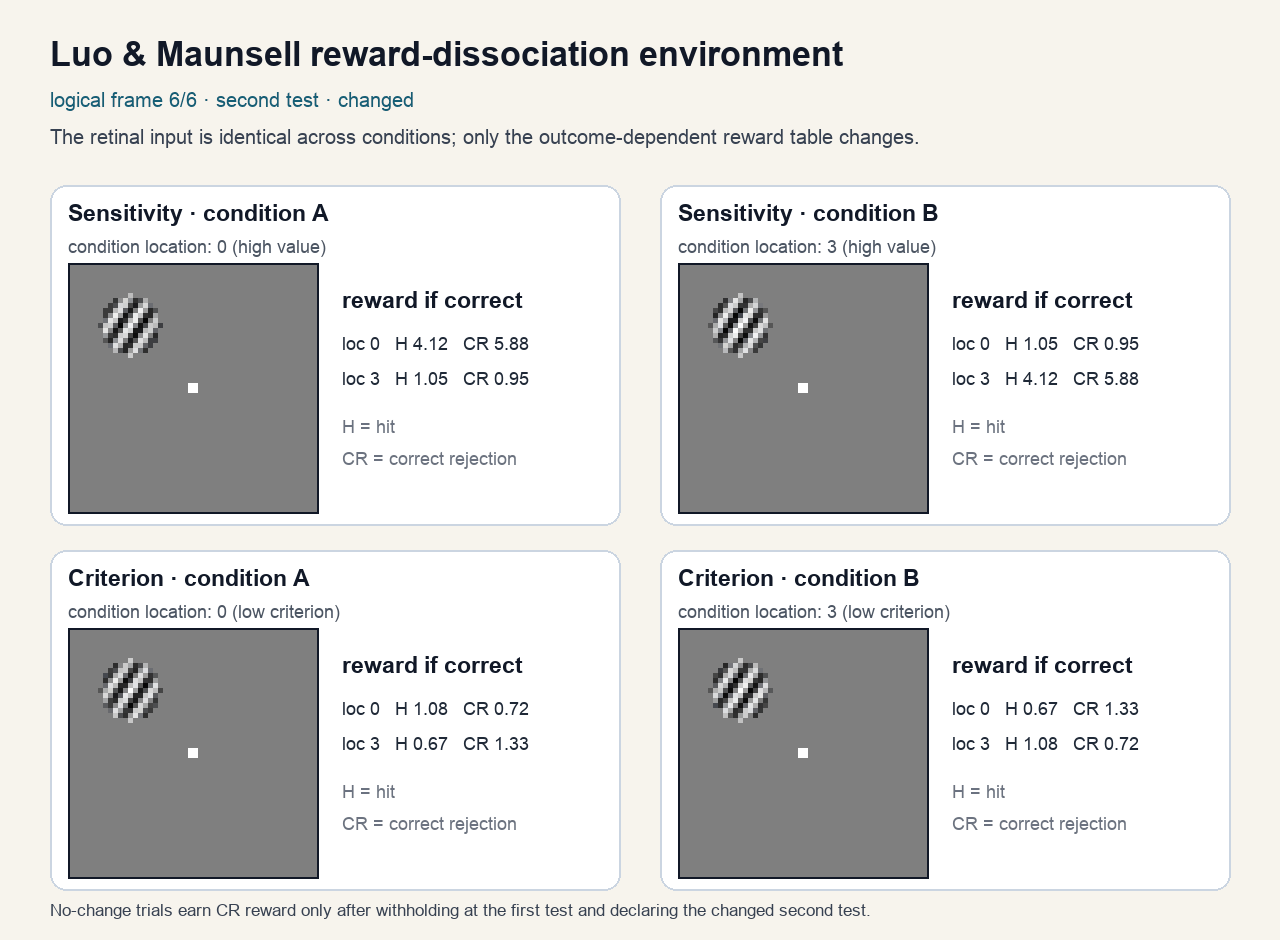
\includegraphics[width=0.91\linewidth]{luo_maunsell_protocol_frame_6.png}
\caption{Changed second test on a no-change trial. A declaration here completes the correct-rejection sequence and releases the location- and outcome-specific CR reward.}
\label{fig:second}
\end{figure}
\clearpage

\section{Verification evidence}

\begin{itemize}
\item \textbf{Focused tests:} all 21 environment-protocol cases and 20 paired-experiment cases passed (41 total). They cover reward means/ratios and counterphasing, event semantics, separate offline exclusion categories, rendering, checkpoint compatibility, fixed-condition matrix construction, immutable embedded parent lineage, strict warm starts and resume roots, restart manifests, held-out competence-gate cells, protocol drift rejection, matched evaluation banks, canary-analysis rejection, and difference-in-differences signs.
\item \textbf{Live outcome exercise:} both registered tasks produced every terminal outcome under deterministic binary action schedules. Using 0 for wait and 1 for declare, the decisive traces were hit $[0,0,0,1]$, miss $[0,0,0,0,0]$, false alarm $[0,0,0,1]$, correct rejection $[0,0,0,0,0,0,1]$, immediate fixation break $[1]$, and second-test miss $[0,0,0,0,0,0,0]$. Additional declarations at frames 1, 2, and 5 confirmed the remaining reachable fixation-break transitions. The emitted rewards matched the explicit tables above.
\item \textbf{Syntax:} \code{envs/luo2015.py}, the analysis module, trainer, rendering script, and tests compiled with the active Python interpreter.
\item \textbf{Broader suite:} 312 passed, 3 failed, 88 warnings in 80.54 seconds. The failures are outside the modified Luo paths and arise because the active Python 3.9 lacks \code{Path.hardlink_to} and \code{zip(..., strict=True)} used by unrelated matched-width and VDA figure tests.
\item \textbf{GIF QA:} the generated GIF is 1280$\times$940, seven frames, 475,625 bytes. Sample, delay, first test, gap, and second test were verified. Full-frame inspection found no clipping, overlap, or condition-dependent visual cue.
\item \textbf{Training canary:} one equal-reward parent and four condition-specific child cells completed on MPS, strictly restored all parent weights (87 loaded, 0 skipped), embedded the same verified parent SHA-256 in every child, used $\gamma=1$, and passed independent task/reward/theta/curriculum/iteration/producer-hash contracts. Each cell wrote rolling and final saves, so these five logical cells correspond to ten physical checkpoint files. A second launcher invocation skipped all five completed cells. The explicit canary bypass is plumbing evidence only, and the analyzer rejects it as behavioral input.
\end{itemize}

\section{What is now valid---and what is not}

\colorbox{good}{\parbox{0.96\linewidth}{
\textbf{Valid now:} the repository has a corrected seven-frame transition analogue and a paired finite-budget optimization path using the existing VDA architecture and PAC/QR-DQN/JEPA trainer. Each seed creates one equal-reward parent and four fixed-condition children with identical inherited model weights at the fork, no reward cue, matched budgets, immutable embedded lineage, source/protocol validation, a balanced held-out parent gate, common evaluation trials, and counterphased contrasts. The analyzer preserves separate exclusion categories by location/status.
}}

\colorbox{warn}{\parbox{0.96\linewidth}{
\textbf{Still required for a local behavioral claim:} first encode and test the numerical child denominator, exclusion, saturation, failed-seed, uncertainty, directional-decision, and equivalence rules stated above; preregister or otherwise timestamp that immutable contract; use an evaluation seed independent of every parent-gate seed; and evaluate robustness across multiple independently drawn orientation-base pairs. Only then run the full paired-seed matrix, pass every equal-reward-parent gate, and estimate the prespecified contrasts. Canary checkpoints are deliberately too short for any behavioral claim.
}}

\subsection{Why continuous learning is not required}

The core computational question can be posed as a finite-budget optimization comparison: does a fixed reward schedule produce the predicted directional difference between trained policies? A recurrent state spanning trials is unnecessary for that estimand. For each seed, the launcher first trains one equal-reward perceptual parent, then forks its exact model weights into sensitivity/criterion $\times$ location-0/location-3 children. The condition and reward table remain fixed during each child's ordinary episodic updates. Thus reward feedback changes network parameters across episodes; the policy never needs to infer an unobserved block switch within its recurrent state.

This design is more controlled than agents trained from unrelated random initializations. Children are paired by parent model state, architecture, seed, difficulty, and budget, while trainer-owned state starts fresh. Global positive scaling sets the arithmetic mean of the four correct-outcome reward magnitudes to one within each session type while retaining every reward ratio; it does not normalize behavior-weighted expected return. Planned runs use $\gamma=1$ because hit rewards can occur at the first test while correct-rejection rewards occur at the second; false alarms receive zero. Discounting would otherwise alter the intended H:CR incentive. A full run has one hard gate before children launch: the equal-reward parent must reach target $\theta$, then achieve 75\% accuracy and 90\% valid engagement separately for change/no-change trials at both locations on a deterministic balanced bank at that $\theta$.

For any metric $m$, the counterphased estimand is
\[
\Delta_{\mathrm{DID}}(m)=\tfrac12\{(m_0-m_3)_{\mathrm{condition\,0}}-(m_0-m_3)_{\mathrm{condition\,3}}\}.
\]
The prespecified directional predictions are $\Delta_{\mathrm{DID}}(d')>0$ in sensitivity sessions and $\Delta_{\mathrm{DID}}(c)<0$ in criterion sessions. No confirmatory error rate, minimum effect, or equivalence bound is currently encoded. Cross-metric contrasts can therefore be shown descriptively, but claiming ``no effect'' requires a declared equivalence bound rather than a nonsignificant test.

A continuously stateful agent is needed only for a different claim about learning a hidden block switch, adaptation speed, or trial-history effects. The episodic experiment instead tests a fixed-schedule, finite-budget reward-optimization analogue without pretending to reproduce that temporal-learning question. No visible condition cue is introduced.

Because one default evaluation bank contains only one independently drawn orientation-base pair per location, a positive result on that bank alone does not establish generalization over session orientations. Production evidence must include either multiple timestamped, prespecified banks with independently drawn bases or an equivalent hierarchical orientation-bank analysis.

No claim about V4 or LPFC neural modulation follows from the environment alone. The eight obsolete preliminary battery weight files have been deleted. Their retained aggregate logs are historical records only and must not be relabeled as corrected Luo--Maunsell results.

\section{Artifacts and integrity}

\begin{tabularx}{\linewidth}{@{}p{0.28\linewidth}Y@{}}
\toprule
Artifact & SHA-256 \\
\midrule
2015 full paper PDF & \code{fe840430b5e63fa8b043a327b2960a1d2981ae2a792109bf3feeb48fc56608d8} \\
2015 supplement PDF & \code{4cb6fc4fd7b36452f7540cbde66691aa33d50278aa0b1e12d9d52038d9f9e391} \\
2018 full paper PDF & \code{9d9b9e341adc4bfc65811b653f4ce051fa8c215f12233b52b4ebdc19df9e2b14} \\
2018 supplement PDF & \code{7a245fcd73475bd142029cc06f762559f89199225ba7adef57bf5e3829d88386} \\
Protocol GIF & \code{9143ecb69697ab72313978bd6ac973f830c58121a33de2d08fbb0e30bb4f6ccd} \\
Corrected environment source & \code{9128d7d54ea8c33b8e037d244ece9e0163a1d73c5b5dc6ebea944602162c7f4c} \\
RL trainer with lineage contract & \code{761f9632c8be6413b93574a3f36ab51eb8101d6c9abeb8ec214826816272255b} \\
Episodic matrix launcher & \code{fb9eaff5607673116f837002c6a5acd8d61748bb0d1a0b9a04cf862837a8911e} \\
Paired SDT analyzer & \code{62292524a5d6e8dfb4ac64fba97e23493bc56f58c728843ce5d9753909132739} \\
SDT classification core & \code{5818662697d26ee1f02b8595bd739fe0f9d315c12546e81e733d2794f3ee6b45} \\
Experiment contract README & \code{9f49d628d8d6bed61c0cc71d0aaf4aa82942ad355a6f2f5ae8054015815b873f} \\
Canary manifest & \code{6f5d83a1a2559dcad60184cd81d0755a643ac9fb634c6d1185e6d1f4d0c2e74b} \\
\bottomrule
\end{tabularx}

Artifact paths are relative to \path{/Users/jonathanmorgan/AttentionManuscript}:
\begin{itemize}[itemsep=1pt,topsep=2pt]
\item Papers: \path{reports/luo_maunsell_environment/papers/}; animation: \path{reports/luo_maunsell_environment/luo_maunsell_protocol.gif}.
\item Code root: \path{RViT_plus_paper_jepa_grid9/}. Code rows map to \path{envs/luo2015.py}, \path{train_rl.py}, \path{experiments/luo2015_episodic/run_matrix.py}, \path{experiments/luo2015_episodic/analyze_matrix.py}, \path{luo2015_analysis/luo2015_core.py}, and \path{experiments/luo2015_episodic/README.md}.
\item Canary manifest under that code root: \path{runs/luo2015_episodic_canary/experiment_manifest.json}.
\end{itemize}

\section*{Primary sources}
\begin{enumerate}[leftmargin=1.4em]
\item Luo, T. Z., \& Maunsell, J. H. R. (2015). Neuronal modulations in visual cortex are associated with only one of multiple components of attention. \emph{Neuron}, 86(5), 1182--1188. \href{https://doi.org/10.1016/j.neuron.2015.05.007}{doi:10.1016/j.neuron.2015.05.007}. PMCID: PMC4458699. Task timing and reward logic are in the main Methods (``Dissociation Task'' and ``Reward Manipulations'') and Supplemental Experimental Procedures (``Dissociation Task--Reward Procedures,'' ``Priming Trials,'' and ``Choice of Reward Parameters'').
\item Luo, T. Z., \& Maunsell, J. H. R. (2018). Attentional changes in either criterion or sensitivity are associated with robust modulations in lateral prefrontal cortex. \emph{Neuron}, 97, 1382--1393.e7. \href{https://doi.org/10.1016/j.neuron.2018.02.007}{doi:10.1016/j.neuron.2018.02.007}. PMCID: PMC5866245. Used only for the related LPFC context, not as the local task specification.
\end{enumerate}

\end{document}
